\documentclass{article} % For LaTeX2e
\usepackage[final]{colm2026_conference}

\usepackage{microtype}
\usepackage[table]{xcolor}
\usepackage{hyperref}
\usepackage{url}
\usepackage{booktabs}
\usepackage{graphicx}
\usepackage{tabularx}
\usepackage{array}
\usepackage[capitalise]{cleveref}
\crefname{table}{Tab.}{Tabs.}
\crefname{figure}{Fig.}{Figs.}
\crefname{section}{Sec.}{Secs.}

\definecolor{darkblue}{rgb}{0, 0, 0.5}
\hypersetup{colorlinks=true, citecolor=darkblue, linkcolor=darkblue, urlcolor=darkblue}
\definecolor{labours}{HTML}{EDEDED}
\newcommand{\ci}[2]{{\scriptsize[#1, #2]}}
\newcommand{\pmstd}[2]{#1{\scriptsize\,$\pm$\,#2}}
\newcolumntype{L}[1]{>{\raggedright\arraybackslash}p{#1}}
\newcolumntype{Y}{>{\raggedright\arraybackslash}X}

\title{One-head attention pooling adds little beyond a deeper MLP in a Qwen2.5-VL region probe}

\author{Khai-Nguyen Nguyen \\
University of Virginia, DS 7400 Homework 3 \\
\url{https://github.com/nkn002/visual-readout}}

\begin{document}

\maketitle
\lhead{DS 7400 Deep Learning, Homework 3 experiment report}

We test whether attention pooling over the tokens under a box improves the HW2 probe, which names a Visual Genome box's content from Qwen2.5-VL-7B's hidden state 21.
Our design (one-head attention and a two-hidden-layer MLP) beats HW2 by +0.71 points, but the same MLP on the mean pool already gains +0.48.
Eight heads gain about one point, yet part of that gain appears on one-token boxes, where attention cannot act, and person recall does not improve.

\section{Hypothesis, committed before training}
\label{sec:hyp}

\textbf{Problem.} The HW2 probe averages the $L$ tokens under a box and feeds the 3,584-d mean to an MLP (3584 $\to$ 512 $\to$ ReLU $\to$ 20) that predicts one of 20 categories.
Its weakest category is person (50\% recall), whose boxes often show mostly a shirt, a face, or an arm.

\textbf{Design.} We replace the mean with attention pooling and add a second hidden layer (3584 $\to$ 512 $\to$ ReLU $\to$ 512 $\to$ ReLU $\to$ 20).
The pooled vector is $\sum_i a_i x_i$ with $a_i = \mathrm{softmax}_i\big(q^\top W_k \hat{x}_i / \sqrt{64}\big)$, where $x_i$ are the tokens under the box and $\hat{x}_i$ their standardized values.
The query $q$ starts at zero, so training starts from the exact mean pool.
An 8-head variant gives each head its own query and its own 448-d slice of the vector.

\textbf{Predictions.} Learned weights can favor object tokens over background tokens.
Before any arm trained (commit \texttt{c03e240} at 15:02; first result at 15:37), we predicted:
(P1) no change on one-token boxes;
(P2) gains for boxes of 10 or more tokens, growing with size;
(P3) the largest recall gains for person, limb, and clothing;
(P4) a second hidden layer on the mean pool adds overfitting, not accuracy; and
(P5) 8 heads match or beat 1 head.
We also named four failure modes, F1 to F4 (\cref{tab:check}).

\section{Setup}
\label{sec:setup}

We cross pooling (mean, attention with 1 head, attention with 8 heads) with depth (1 or 2 hidden layers) on the HW2 split of 50,000 regions (2,500 per category; 39,968 train, 5,075 validation, and 4,957 test, split by image).
Every arm searches the same grid (Adam; learning rate \{3e-4, 1e-3\} $\times$ weight decay \{1e-4, 1e-3\}; batch 256; dropout 0.5; early stopping), keeps its best setting on validation accuracy, and reruns it with 3 seeds.
We score the test set once per arm and report paired-bootstrap 95\% CIs over test regions, which leave out training-seed variance.
The 843 one-token test boxes act as a placebo: there attention returns the token itself, so the pooled input equals HW2's.

\section{Results}
\label{sec:results}

\begin{table}[t]
\centering
\caption{The proposed design (gray) beats HW2 by +0.71 points, but depth alone gives +0.48. Test accuracy (\%) is the mean $\pm$ std over 3 seeds; $\Delta$ is the gain in points with its 95\% CI.}
\label{tab:main}
\small
\setlength{\tabcolsep}{3.5pt}
\begin{tabular}{@{}llcccr@{}}
\toprule
Pooling & Hidden & Test acc. & $\Delta$ vs.\ HW2 & $\Delta$ vs.\ mean, same depth & Epoch (s) \\
\midrule
Mean (HW2) & 1 & \pmstd{73.62}{0.38} & -- & -- & 0.09 \\
\midrule
Mean & 2 & \pmstd{74.10}{0.21} & +0.48 \ci{+0.01}{+0.95} & -- & 0.21 \\
Attention, 1 head & 1 & \pmstd{74.10}{0.15} & +0.48 \ci{$-$0.09}{+1.06} & +0.48 \ci{$-$0.09}{+1.06} & 0.77 \\
\rowcolor{labours} Attention, 1 head & 2 & \pmstd{74.33}{0.08} & +0.71 \ci{+0.05}{+1.32} & +0.24 \ci{$-$0.40}{+0.80} & 0.69 \\
Attention, 8 heads & 1 & \pmstd{74.48}{0.17} & +0.86 \ci{+0.26}{+1.43} & +0.86 \ci{+0.26}{+1.43} & 1.09 \\
Attention, 8 heads & 2 & \pmstd{\textbf{75.07}}{0.25} & +1.45 \ci{+0.82}{+2.06} & +0.97 \ci{+0.40}{+1.52} & 1.23 \\
\bottomrule
\end{tabular}
\end{table}

\begin{figure}[t]
\centering
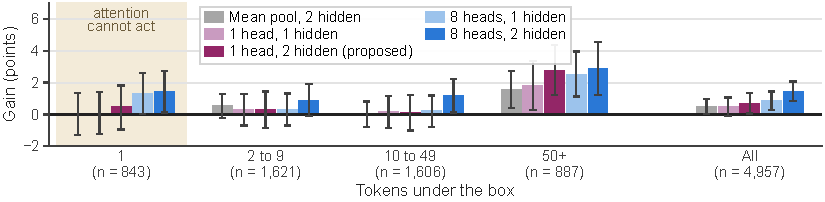
\includegraphics[width=\textwidth]{fig_gain_by_box_size.pdf}
\caption{Part of the 8-head gain appears on one-token boxes, where attention cannot act (shaded). Bars give the test-accuracy gain over HW2 per bin of tokens under the box (3-seed mean); whiskers give 95\% CIs.}
\label{fig:bins}
\end{figure}

\textbf{The second hidden layer, not one-head attention, carries most of the proposed design's gain.}
The proposed design beats HW2 by +0.71 points (\cref{tab:main}).
Yet the same MLP on the mean pool already gains +0.48, so one-head attention adds only +0.24 at the same depth, with a CI that includes zero.
In contrast, eight heads beat the mean pool at both depths (+0.86 and +0.97), and the best arm reaches 75.07\%.

\textbf{One head gains where predicted, but eight heads also gain where attention cannot act.}
At HW2's depth, one head gains +0.08 points on one-token boxes and +1.80 on boxes of 50 or more tokens (\cref{fig:bins}), as P1 and P2 predicted.
However, depth alone also gains +1.54 on these large boxes.
Interestingly, eight heads at HW2's depth gain +1.30 \ci{+0.04}{+2.61} on one-token boxes, where their input equals HW2's, more than their +0.77 on larger boxes.
This borderline result (one of about 30 box-size contrasts) suggests that part of the eight-head gain comes from the jointly trained MLP or from seed variance (HW2's seeds span 73.09\% to 73.90\%), not from re-weighting tokens.

\textbf{Attention does not fix person recall.}
Person recall changes by $-$2.3 points \ci{$-$5.9}{+1.2} for the proposed design and by $-$0.3 for the best arm, while clothing, window and door, street and road, and furniture gain.
The weights stay diffuse (normalized entropy 0.90 to 0.95, where 1 is uniform), and attention costs 3 to 12$\times$ more time per epoch.

\textbf{Conclusion.} Our design gains +0.71 points over HW2, mostly through its second hidden layer, and does not fix person recall (\cref{tab:check}).
Re-scoring each attention probe with uniform weights (not run) would separate the pooling from the jointly trained MLP, and more seeds would put seed variance into the CIs.



\begin{table}[!h]
\centering
\caption{The data support P5, partly support P2 and P4, contradict P1 for eight heads, and do not support P3 for person. Brackets give 95\% CIs in points.}
\label{tab:check}
\small
\setlength{\tabcolsep}{3.5pt}
\begin{tabularx}{\textwidth}{@{}L{1.62in}YL{0.98in}@{}}
\toprule
Prediction or failure mode & Observation & Verdict \\
\midrule
P1. 1-token boxes unchanged & 1 head +0.08; 8 heads +1.30 \ci{+0.04}{+2.61} & Only for 1 head \\
P2. Gain grows with box size & 50+ tokens: attention +1.8 to +2.9; depth +1.5 & Partly; depth too \\
P3. Person, limb, clothing & Person $-$2.3; clothing +3.2 and +6.8 & Not for person \\
P4. Depth: overfitting only & Train 86.4\% vs.\ 82.4\%; test +0.48 \ci{+0.01}{+0.95} & Partly refuted \\
P5. 8 heads $\geq$ 1 head & +0.38 (1 hidden); +0.73 \ci{+0.24}{+1.23} (2 hidden) & Supported \\
\midrule
F1. Weights stay uniform & Entropy 0.90 to 0.95 (1 is uniform) & No; diffuse \\
F2. Position lock & First token on top: 15 to 18\% vs.\ 13 to 14\% & Weak at most \\
F3. Overfitting & Train-val.\ gap 9.4 (HW2), 13.3 (8 heads, 1 hidden) & In one arm \\
F4. Decay, outliers, scaling & Not measured & Not tested \\
\bottomrule
\end{tabularx}
\end{table}

\end{document}
